\section{Durchführung}
\label{sec:Durchführung}

Die Versuchsdurchführung ist zweigeteilt. Zunächst erfolg das Aufnehmen der
Messwerte für eine Schar von fünf Kennlinien, mit dessen Hilfe die Sättigungsströme 
ermittelt und das Langmuir-Schottky’sche Raumladungsgesetz bestimmt werden kann.

\subsection{Bestimmung der Kennlinien}
\label{sec:1}
Es soll eine Schar von fünf verschiedenen Kennlinien dargestellt werden, 
also für jeweils fünf verschiedene Heitzspannungen. Die Schaltung wird gemäß
\autoref{sec:refdufotze} aufgebaut, welche auch in \autoref{fig:11} dargestellt ist.
Die Vakuum-Diode ist an einen Heizspannungs- und Stromgenerator angeschlossen.
Wird dort eine Spannung eingestellt, beginnt die Kathode und damit das Wolfram
zu glühen und es treten Elektronen aus.
Zusätzlich wird an die Diode mit einer weiteren Spannnungsquelle eine Spannung
angelegt, die sogenannte \glqq Absaugspannung\grqq{}. Diese wird kontinuirlich
in kleinen Schritten erhöht und jeweils gegen den gemessenen Absaugstrom
aufgetragen.
\begin{figure}[H]
    \centering
        \centering
        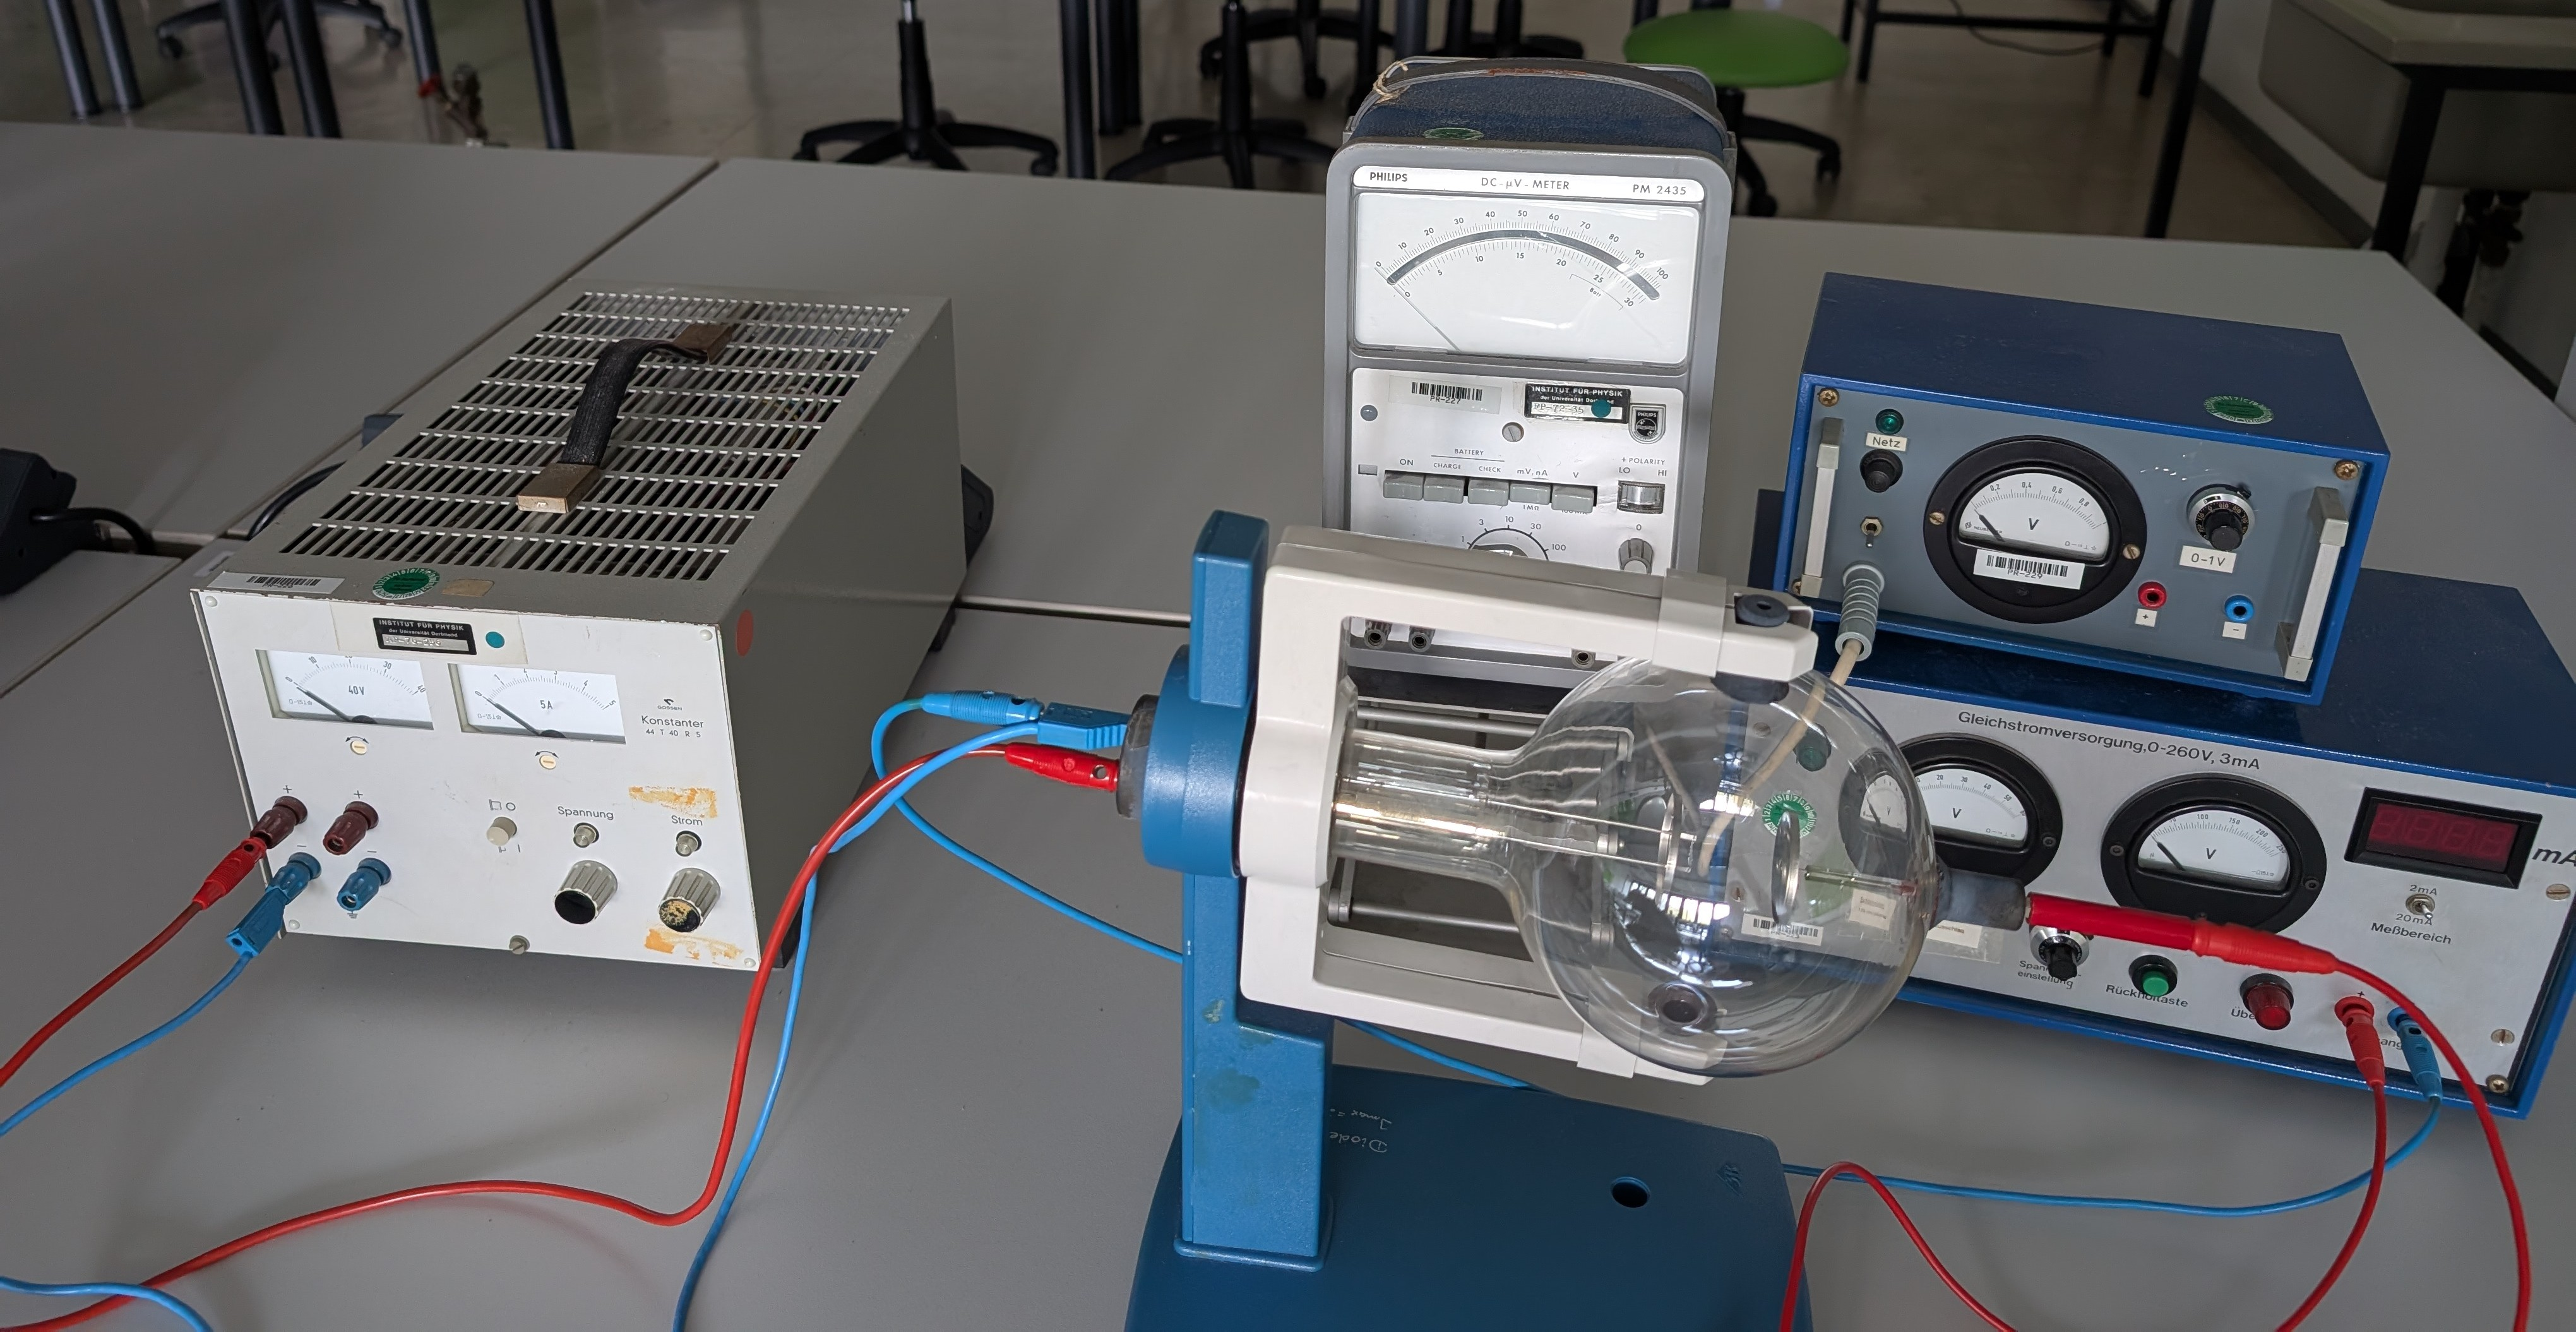
\includegraphics[width=0.8\textwidth]{Bilder/2.jpg}
        \caption{Aufbau-Teil 1.}
    \hfill
    \label{fig:11}
\end{figure}

\subsection{Das Anlaufstromgebiet}
Um den Bereich des Anlaufstromgebiets festzulegen wird die in \autoref{fig:12}
abgebildete Schaltung aufgebaut. Der Aufbau unterscheidet sich von der Schaltung
in \autoref{sec:1} dadurch, dass nun ein invertiertes Gegenfeld kleinerer Spannung
$\left(1 - 2\unit{\volt}\right)$ an die Vakuum Diode angeschlossen wird.
Nun wird eine Heizspannung eingestellt und die Spannung des Gegenfeldes
von Null bis Zehn Volt in verschiedenen Schrittgrößen erhöht und der Anlaufstrom
abgelesen.
\begin{figure}[H]
    \centering
        \centering
        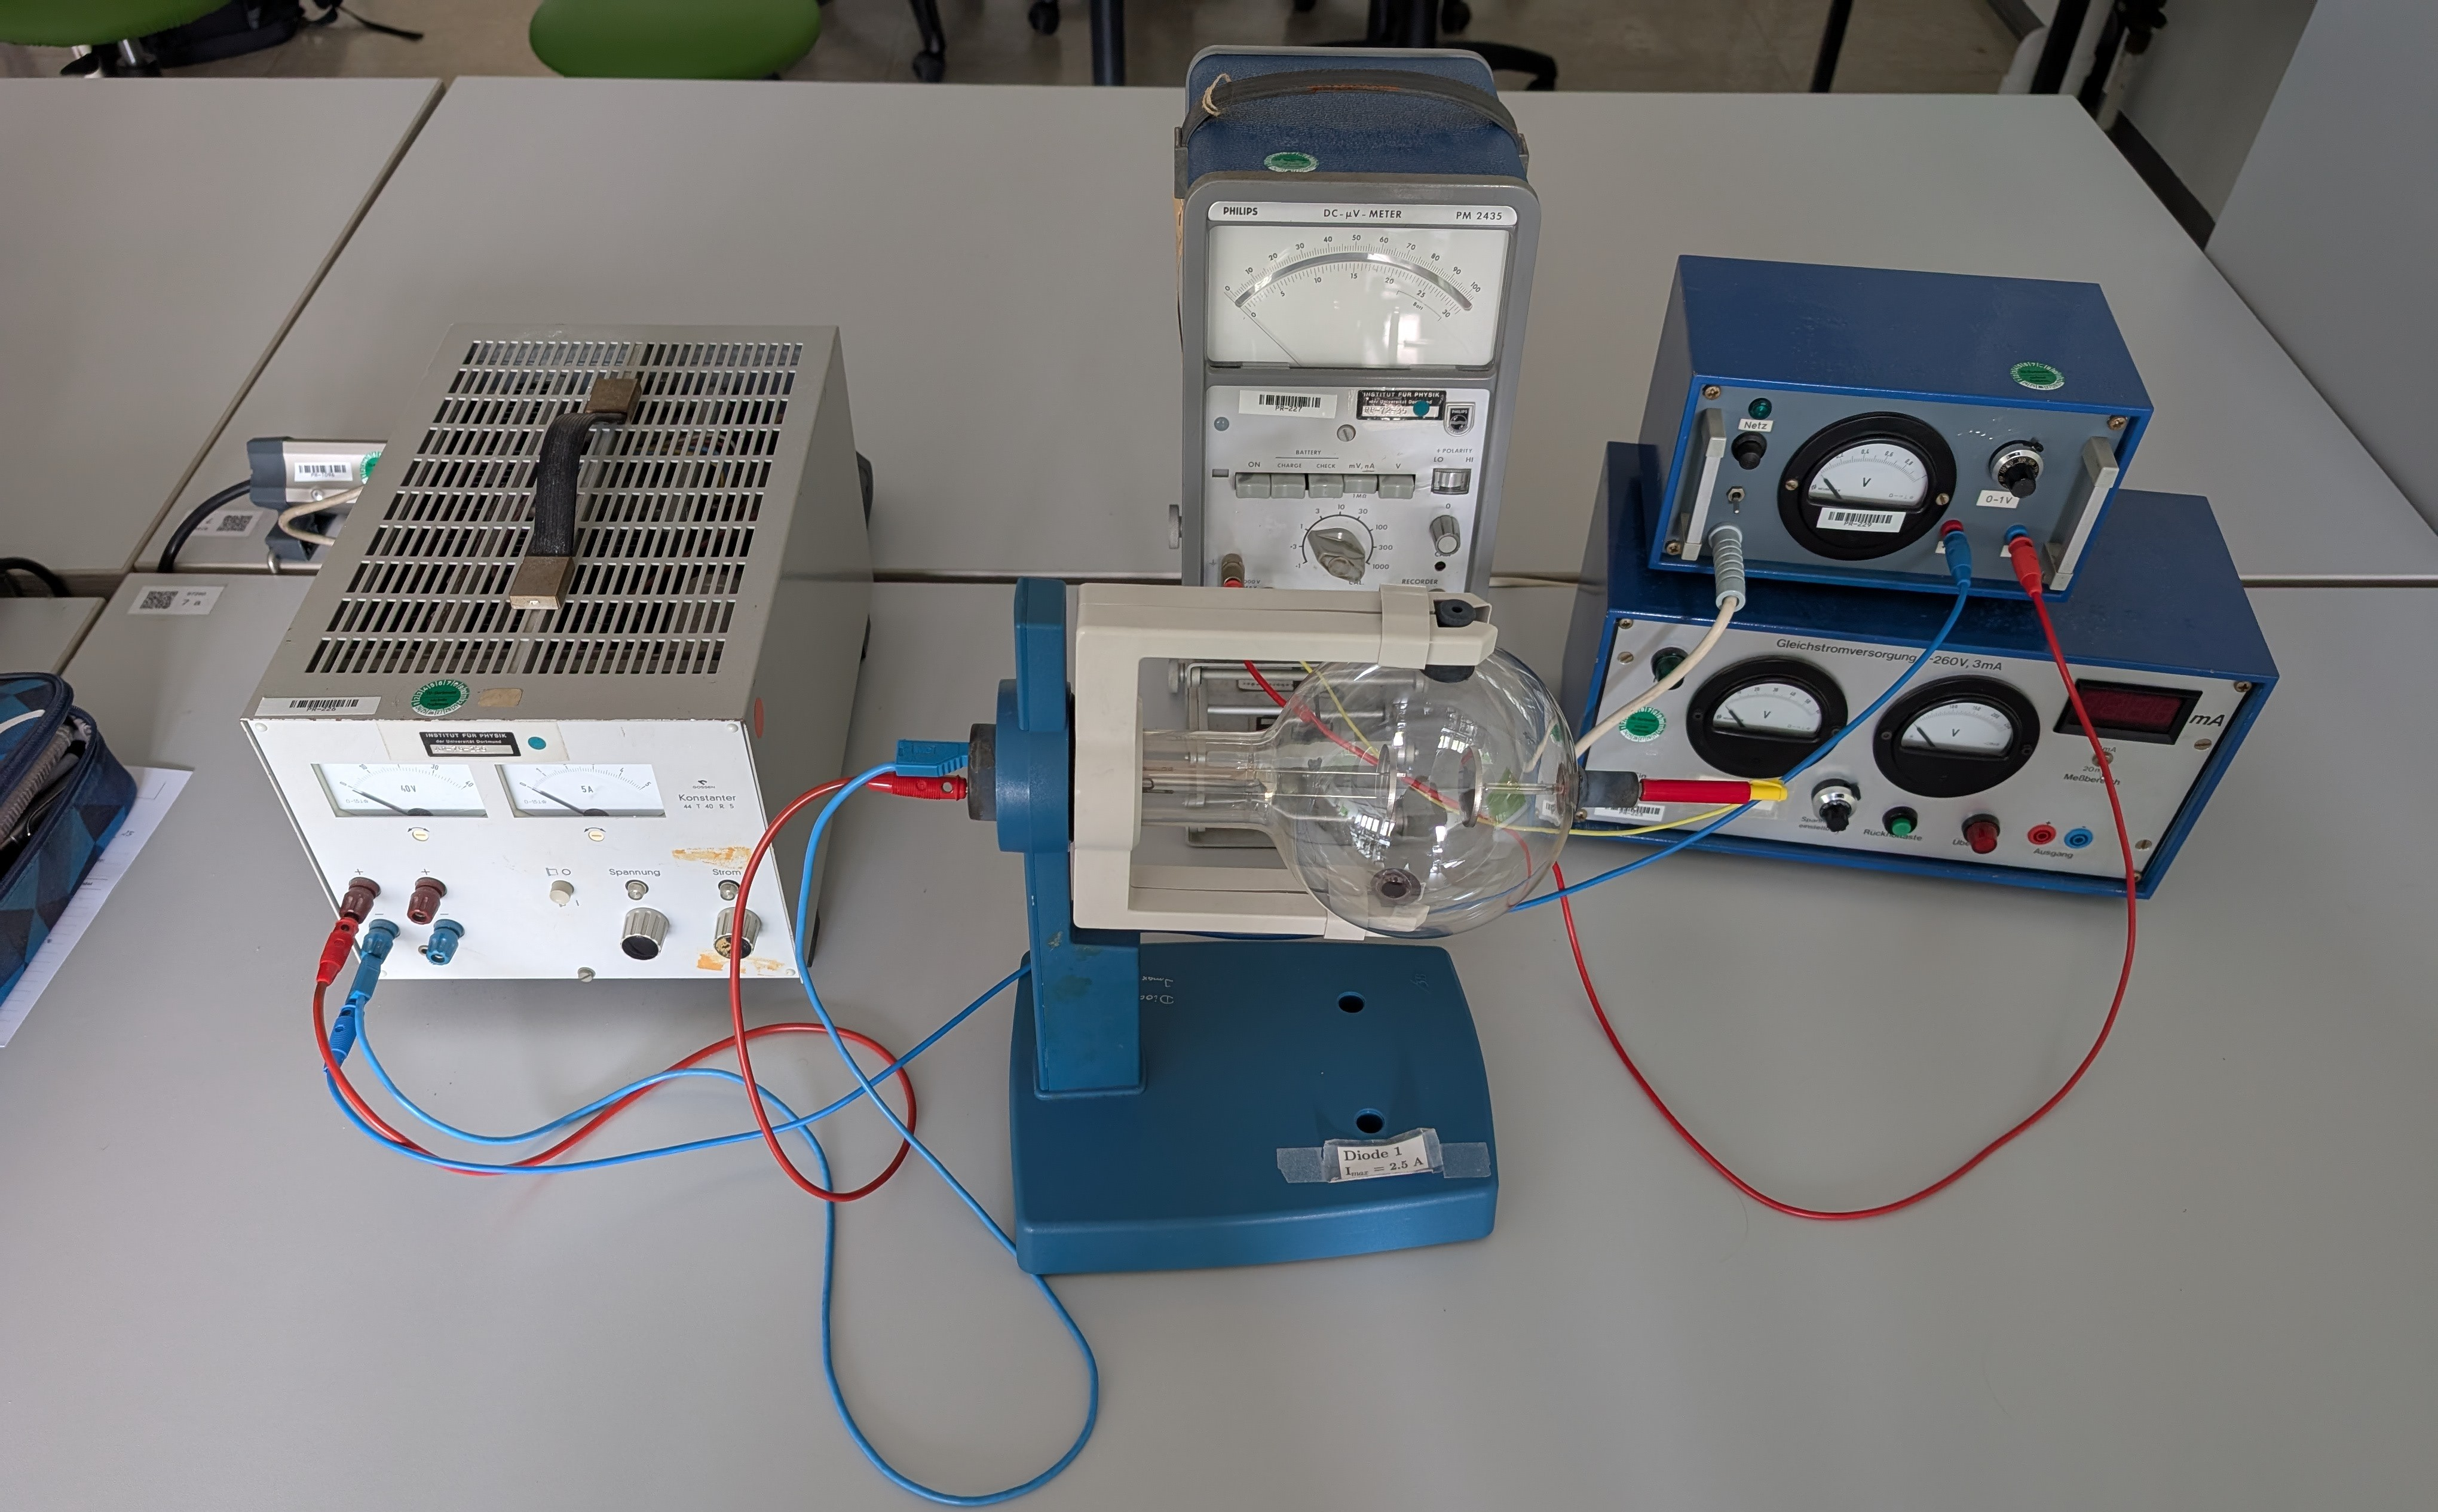
\includegraphics[width=\textwidth]{Bilder/1.jpg}
        \caption{Aufbau-Teil 2.}
    \hfill
    \label{fig:12}
\end{figure}